\documentclass[11pt]{article}
\usepackage{icmlko}
\begin{document}

\title{나라만 다른 손님을 불렀더니 안 통했다 --- 다섯 번째 설명을 묻는다}
\author{월드모델 실험실}
\date{노트 440 · 2026년 8월 6일}
\maketitle

\begin{abstract}
노트 $435 \sim 438$ 이 네 번 연달아 같은 처방에 이르렀다 --- \emph{같은 계기 ·
같은 절차인데 하나만 다른 도메인.} \textbf{CN 만화가 정확히 그것이었다}:
\texttt{manga\_records} 의 같은 수집 · 같은 라벨 계기이고 \texttt{country} 만
다르다. 2025년 이후가 19행이라 접어 뒀었는데, \textbf{판의 만화 도메인이
JP 전용}이므로 \textbf{352행 전부가 안 본 행}이다 --- 시기로 자를 이유가
없었다.

\begin{center}
\begin{tabular}{lrrrr}
\hline
 & 행 & 무표지 & grp & 이득 \\
\hline
KR 만화 · 2025$+$ & $322$ & $-0.0631$ & $+0.2077$ & $\mathbf{+0.2708}$ \\
KR 만화 · 전 연도 & $1{,}716$ & $+0.2330$ & $+0.5015$ & $\mathbf{+0.2685}$ \\
\textbf{CN 만화 · 전 연도} & $352$ & $+0.2249$ & $+0.2713$ & $\mathbf{+0.0465}$ \\
\hline
\end{tabular}
\end{center}

\textbf{CN 은 KR 의 5분의 1이다.} 그런데 \textbf{무표지 팔은 거의 같은
자리에서 출발한다}($+0.2249$ 대 $+0.2330$) --- 공유 축은 둘에게 똑같이
작동하고 \textbf{grp 만 KR 을 크게 들어올린다}.

\textbf{국가 · 언어가 아니다.} 다섯 번째 설명이 죽는다.
\end{abstract}

\section{덤으로 얻은 것 --- KR 의 값은 규약을 안 탄다}

이 실험이 부수적으로 이 사이클의 중심 수치를 검사했다. KR 만화의 grp 이득이
\textbf{2025$+$ 322행에서 $+0.2708$, 전 연도 1{,}716행에서 $+0.2685$} 다.
행 집합도 절대 수준도 완전히 다른데(무표지가 $-0.06$ 대 $+0.23$) \textbf{틈은
같다.}

노트 417부터 이 사이클이 기대 온 수치가 \textbf{채점 규약의 부산물이
아니다}. 노트 430이 ``KR 은 평범한 손님''임을 보인 데 이어 두 번째 검사다.

\section{다섯이 죽었다 --- 관측으로 둔다}

\begin{center}
\begin{tabular}{lll}
\hline
설명 & 잰 값 & 노트 \\
\hline
거리 & $\rho = -0.203$, 집 밖이 더 가깝다 & 435 \\
축 수 --- 예보 & $\rho = -0.451$, 집안만 $-0.248$ & 436 \\
축 수 --- 빼기 & 이득 증가의 $62\%$ 가 바닥 붕괴 & 437 \\
축 수 --- 붙이기 & $7 \to 13$ 인데 이득 불변 & 438 \\
\textbf{국가 · 언어} & \textbf{CN $+0.047$ 대 KR $+0.269$} & 여기 \\
\hline
\end{tabular}
\end{center}

이 실험실은 이런 자리에 처분이 있다 --- 노트 385가 달력에, 노트 414가 웹툰에
쓴 것.

\begin{center}
\textbf{KR 만화가 grp 에서 유난히 버는 까닭은 관측으로 둔다.}
\end{center}

측정은 튼튼하다: 두 규약에서 같고(여기), 오차 막대가 붙어 있고(노트 418:
$95\%\ [+0.099, +0.312]$, $800/800$), 두 번째 짝에서 부호가 재현된다
(비게임 앱 $+0.105$). \textbf{무엇이 그것을 만드는지 모를 뿐이다.}

\begin{tabular}{lp{7.0cm}}
\hline
CN 도 $+0.047$ 은 된다 & 0 이 아니다. 집안 LODO 평균($-0.0004$)보다는 낫고
KR 보다는 훨씬 못하다 --- \textbf{집 밖이 한 덩어리가 아니다} \\
남은 후보 & KR 과 CN 을 가르는 것: 표본 크기($1{,}716$ 대 $352$) · 연재
형식 · 라벨 분포. 셋 다 안 재 봤다 \\
씨앗 & LODO 쪽 문턱을 내리는 일이 세 노트째 밀려 있다 \\
\hline
\end{tabular}

\begin{figure}[h]
\centering
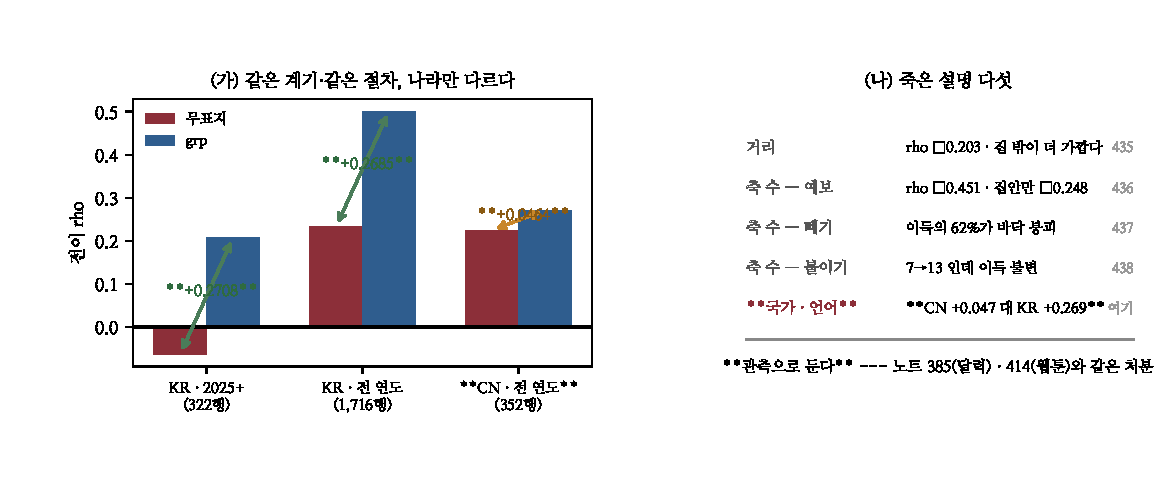
\includegraphics[width=\textwidth]{figs/fig440.pdf}
\caption{(가) 무표지 팔은 같은 자리에서 출발하는데 grp 가 KR 만 들어올린다.
(나) 죽은 설명 다섯.}
\end{figure}

\end{document}
